\section{Overview}
\label{chapter:TypeShild Overview}
In this section, we present in~\cref{TypeShield Policy Mechanism} our type based policy and approach overview in Figure~\ref{System overview.}. 
In~\cref{Backward Edge CFI Policy} we highlight our backward edge protection policy.
% while  
% in~\cref{Invariants for Targets and Callsites} we present the invariants for calltargets and callsites, while 
% in~\cref{Adversary Model} we introduce our threat model.
% Finally, in~\cref{TypeShild Impact on COOP} we talk about parameter count vs. parameter type policies.

% \begin{center}
% \begin{figure*}[t!]
% \centering
%    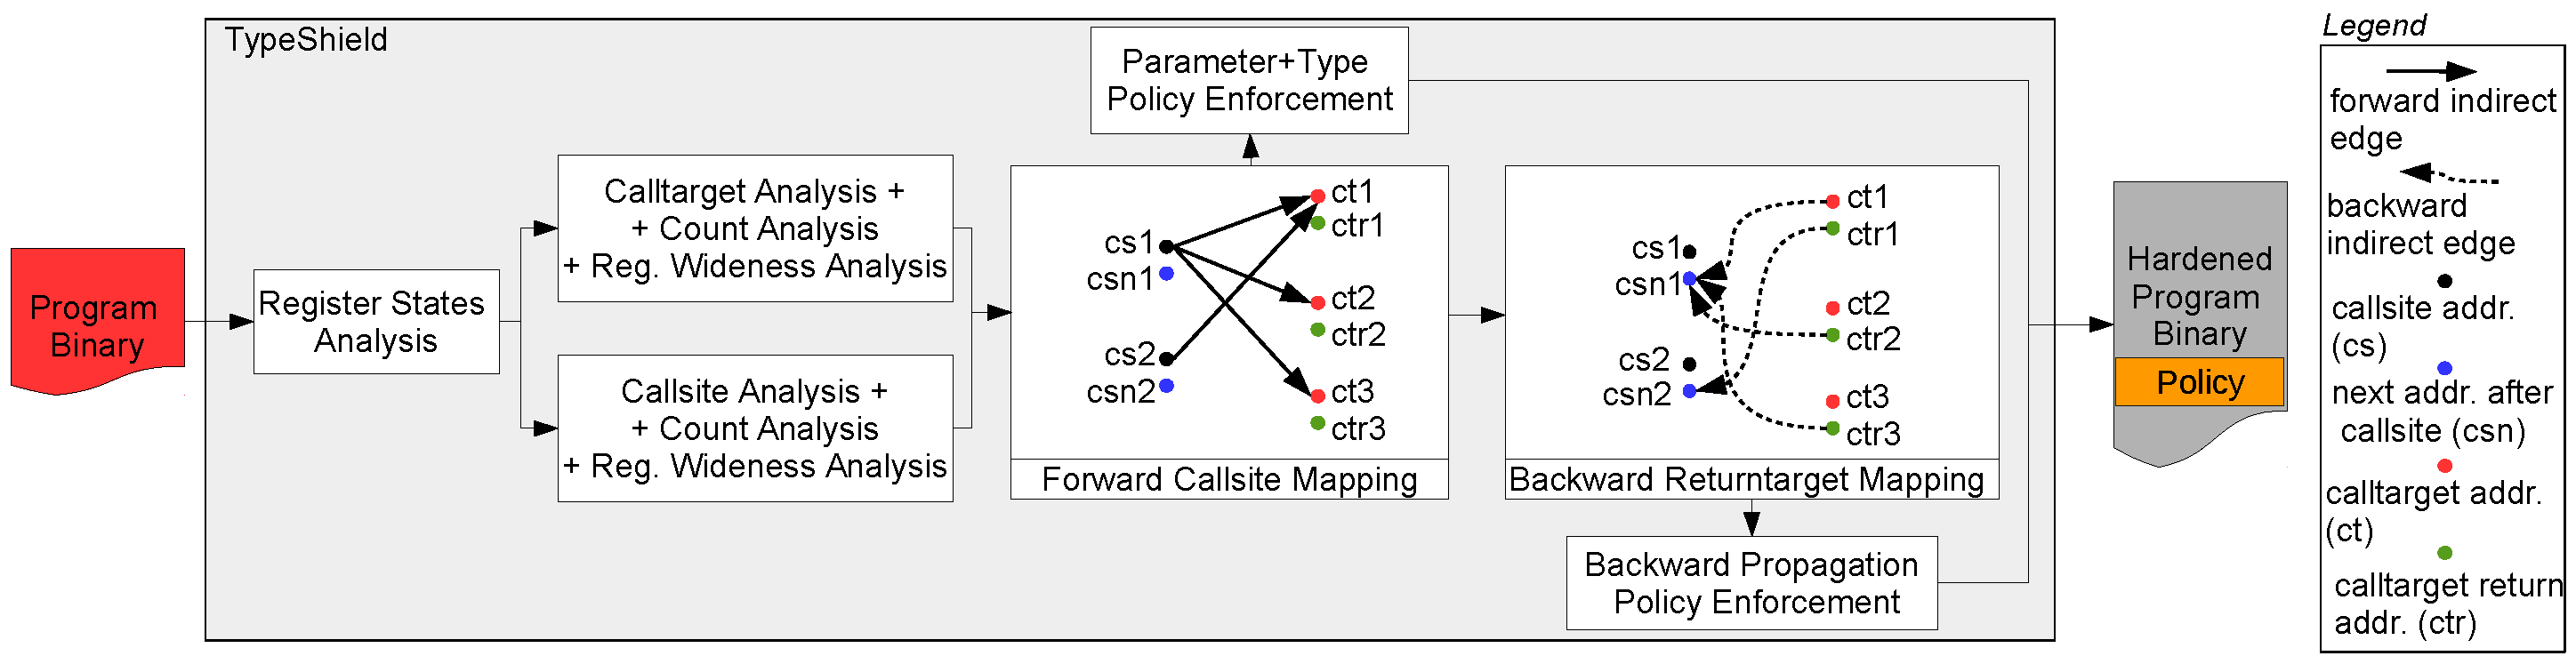
\includegraphics[width=.88\textwidth]{figures/overview.pdf}
%     \caption{Approach overview.
% %     The original program binary is analyzed (see left hand side in above Figure) by \textsc{TypeShield} and the calltargets and callsite analysis are performed for determining how many parameters are 
% %     provided, how many are consumed and their register wideness.
% %     After this step labels are inserted at each previously identified callsite and at each calltarget. 
% %     The enforced policy is schematically represented by the black highlighted dots (addresses) in the above Figure which are allowed to call only legitimate red highlighted dots (addresses).
% %     Next for each function return address the address set determined by each address located after each legitimate (is allowed to call the function) callsite is collected.
% %     This information is obtained by using the previously determined callsite forward-edge mapping to derive a function return backward map containing function returns as key and return targets as values.
% %     In this way \textsc{TypeShield} has for each function return site a set of legitimate addresses where the function return site is allowed to transfer the program control flow.
% %     Finally, range or compare checks are inserted before each function return site. This checks are used to check during runtime if the 
% %     address where the function return wants to jump to is contained in the legitimate set for each particular return site.
% %     This is represented above Figure by green highlighted dots (addresses) that are allowed to call only legitimate blue highlighted dots (addresses).
% %     Finally, the result is a hardened program binary (see right hand side in above Figure).
% }
%     \label{System overview.}
%     \vspace{-.5cm}
%  \end{figure*}
% \end{center}

% \subsection{Invariants}
% % \textbf{Invariants for Targets and Callsites.}
% \label{Invariants for Targets and Callsites}
% 
% \subsubsection{Calltargets and Callsites}
% We propose the following invariants for the function calltargets and callsites.
% (1) indirect callsites provide a number of parameters (\textit{i.e.,} possibly overestimated compared to program source code), 
% (2) calltargets require a minimum number of parameters (\textit{i.e.,} possibly underestimated compared to program source code), and
% (3) the wideness of the callsite parameters has to be bigger or equal to the wideness of the parameters registers expected at the calltarget.
% In a nutshell the idea is that a callsite might only call functions that do not require more parameters than provided by the callsite and
% where the parameter register wideness of each parameter of the callsite is higher or equal to that parameter registers used at the calltarget.
% Figure~\ref{System overview.} depicts this requirements by the forward indirect edges pointing from the black dots to the legitimate
% red dots.
% 
% \subsubsection{Callertarget Returns}
% We propose the following invariant for the calltargets returns.
% (1) we enforce the caller caller convention between the calltarget return instruction and the address next to callsite which was used in first place to 
% call that calltarget.
% Figure~\ref{System overview.} depicts this analogy by the backward indirect edges pointing from the green dots to the legitimate
% blue dots.
% \vspace{-.99cm}
\subsection{Type Based Policy}
\label{TypeShield Policy Mechanism}

\begin{figure}[H]
% \captionsetup{labelformat=empty}
\vspace{-.3cm}
\hspace{-.3cm}
\resizebox{0.49\textwidth}{!}{
\begin{tikzpicture}[shorten >=1pt,node distance=2cm,on grid,auto]
    \begin{scope}
            % labels
%     \foreach \i in {0,...,5}
%       \path[blue] (0,-0.25) node{0} (-0.25,0) node{0};
      \path[blue] (0.25,-0.25) node{1}  (-0.25, 0.25) node{0};
      \path[blue] (0.75,-0.25) node{2}  (-0.25, 0.75) node{1};
      \path[blue] (1.25,-0.25) node{3}  (-0.25, 1.25) node{2};
      \path[blue] (1.75,-0.25) node{4}  (-0.25, 1.75) node{4};
      \path[blue] (2.25,-0.25) node{5}  (-0.25, 2.25) node{8};
      \path[blue] (2.75,-0.25) node{6} (-0.25, 2.75) node{};
%       \path[blue] (7/2,-0.25) node{64} (-0.25,7/2) node{64};
    % loop over the lattice points
    \foreach \i in {0,...,6}
      \foreach \j in {0,...,6}{
       \ifnum \j < 6
        \draw (\i / 2,\j / 2) rectangle (1,1);
        \fi
        % check if (\i,\j) > (2,2)
%         \ifnum \i < 3
%           \ifnum \j < 3
%             \fill[red] (\i + 0.25,\j + 0.25) circle(3pt);
%           \fi
%         \fi
      };
      
      \fill (0   + 0.25, 0   + 0.25) circle(4pt);
      \fill (0.5 + 0.25, 0.5 + 0.25) circle(4pt);
      \fill (0 + 0.25, 0.5 + 0.25) circle(4pt);
      \fill (0.5 + 0.25, 0 + 0.25) circle(4pt);
      \fill (0.5 + 0.25, 1 + 0.25) circle(4pt);
      \fill (0 + 0.25, 1 + 0.25) circle(4pt);
      %       \draw [line width=0.5mm, green] (1 + 0.25, 1 + 0.25) circle (6pt);
      
%       \draw (0.5 + 0.25, 3 + 0.25) circle(4pt);
%       \draw (0 + 0.25, 3 + 0.25) circle(4pt);
%       \draw (1 + 0.25, 3 + 0.25) circle(4pt);
%       \draw (1 + 0.75, 3 + 0.25) circle(4pt);
%       \draw (2.25, 3 + 0.25) circle(4pt);
%       \draw (2.75, 3 + 0.25) circle(4pt);
%       \draw (3.25, 3 + 0.25) circle(4pt);
      
%       \draw (0.5 + 0.25, 2.5 + 0.25) circle(4pt);
%       \draw (0 + 0.25, 2.5 + 0.25) circle(4pt);
%       \draw (1 + 0.25, 2.5 + 0.25) circle(4pt);
%       \draw (1 + 0.75, 2.5 + 0.25) circle(4pt);
%       \draw (2.25, 2.5 + 0.25) circle(4pt);
%       \draw (2.75, 2.5 + 0.25) circle(4pt);
%       \draw (3.25, 2.5 + 0.25) circle(4pt);
      
      \draw (0.5 + 0.25, 2 + 0.25) circle(4pt);
      \draw (0 + 0.25, 2 + 0.25) circle(4pt);
      \draw (1 + 0.25, 2 + 0.25) circle(4pt);
      \draw (1 + 0.75, 2 + 0.25) circle(4pt);
      \draw (2.25, 2 + 0.25) circle(4pt);
      \draw (2.75, 2 + 0.25) circle(4pt);
%       \draw (3.25, 2 + 0.25) circle(4pt);
      
      \fill (0.5 + 0.25, 1.5 + 0.25) circle(4pt);
      \fill (0 + 0.25, 1.5 + 0.25) circle(4pt);
      \fill (1 + 0.25, 1.5 + 0.25) circle(4pt);
      \fill (1 + 0.75, 1.5 + 0.25) circle(4pt);
      \draw (2.25, 1.5 + 0.25) circle(4pt);
      \draw (2.75, 1.5 + 0.25) circle(4pt);
%       \draw (3.25, 1.5 + 0.25) circle(4pt);
      
      \fill (1 + 0.25, 1 + 0.25) circle(4pt);
      \fill (1 + 0.75, 1 + 0.25) circle(4pt);
      \fill (2.25, 1 + 0.25) circle(4pt);
      \fill (2.75, 1 + 0.25) circle(4pt);
%       \draw (3.25, 1 + 0.25) circle(4pt);
      
      \fill (1 + 0.25, 0.5 + 0.25) circle(4pt);
      \fill (1 + 0.75, 0.5 + 0.25) circle(4pt);
      \fill (2.25, 0.5 + 0.25) circle(4pt);
      \fill (2.75, 0.5 + 0.25) circle(4pt);
%       \fill (3.25, 0.5 + 0.25) circle(4pt);
      
      \fill (1 + 0.25, 0 + 0.25) circle(4pt);
      \fill (1 + 0.75, 0 + 0.25) circle(4pt);
      \fill (2.25, 0 + 0.25) circle(4pt);
      \fill (2.75, 0 + 0.25) circle(4pt);
%       \fill (3.25, 0 + 0.25) circle(4pt);
    \end{scope}
    
    \begin{scope}[xshift=1.5cm, yshift=2.75cm]
     \node[]    (q_1) {	\large{$M1:callsite$}};
    \end{scope}
    
    \begin{scope}[xshift=3.25cm, yshift=1.2cm]
     \node[]    (q_1) {	\large{$\wedge$}};
    \end{scope}
    
    \begin{scope}[xshift=5.3cm, yshift=2.75cm]
     \node[]    (q_1) {	\large{$M2:calltarget$}};
    \end{scope}
    
    \begin{scope}[xshift=9cm, yshift=2.75cm]
     \node[]    (q_1) {\large{$M3:policy \ result$}};
    \end{scope}

    \begin{scope}[xshift=3.8cm]
       % labels
%     \foreach \i in {0,...,5}
%       \path[blue] (0,-0.25) node{0} (-0.25,0) node{0};
      \path[blue] (0.25,-0.25) node{1}  (-0.25, 0.25) node{0};
      \path[blue] (0.75,-0.25) node{2}  (-0.25, 0.75) node{1};
      \path[blue] (1.25,-0.25) node{3}  (-0.25, 1.25) node{2};
      \path[blue] (1.75,-0.25) node{4}  (-0.25, 1.75) node{4};
      \path[blue] (2.25,-0.25) node{5}  (-0.25, 2.25) node{8};
      \path[blue] (2.75,-0.25) node{6} (-0.25, 2.75) node{};
%       \path[blue] (7/2,-0.25) node{64} (-0.25,7/2) node{64};
    % loop over the lattice points
    \foreach \i in {0,...,6}
      \foreach \j in {0,...,6}{
      \ifnum \j < 6
       \draw (\i / 2,\j / 2) rectangle (1,1);
      \fi
        
        % check if (\i,\j) > (2,2)
%         \ifnum \i < 3
%           \ifnum \j < 3
%             \fill[red] (\i + 0.25,\j + 0.25) circle(3pt);
%           \fi
%         \fi
      };
      
      \draw (0   + 0.25, 0   + 0.25) circle(4pt);
      \draw (0.5 + 0.25, 0.5 + 0.25) circle(4pt);
      \draw (0 + 0.25, 0.5 + 0.25) circle(4pt);
      \draw (0.5 + 0.25, 0 + 0.25) circle(4pt);
      \draw (0.5 + 0.25, 1 + 0.25) circle(4pt);
      \draw (0 + 0.25, 1 + 0.25) circle(4pt);
      
%       \fill (0.5 + 0.25, 3 + 0.25) circle(4pt);
%       \fill (0 + 0.25, 3 + 0.25) circle(4pt);
%       \fill (1 + 0.25, 3 + 0.25) circle(4pt);
%       \fill (1 + 0.75, 3 + 0.25) circle(4pt);
%       \fill (2.25, 3 + 0.25) circle(4pt);
%       \fill (2.75, 3 + 0.25) circle(4pt);
%       \fill (3.25, 3 + 0.25) circle(4pt);
      
%       \fill (0.5 + 0.25, 2.5 + 0.25) circle(4pt);
%       \fill (0 + 0.25, 2.5 + 0.25) circle(4pt);
%       \fill (1 + 0.25, 2.5 + 0.25) circle(4pt);
%       \fill (1 + 0.75, 2.5 + 0.25) circle(4pt);
%       \fill (2.25, 2.5 + 0.25) circle(4pt);
%       \fill (2.75, 2.5 + 0.25) circle(4pt);
%       \fill (3.25, 2.5 + 0.25) circle(4pt);
      
      \fill (0.5 + 0.25, 2 + 0.25) circle(4pt);
      \fill (0 + 0.25, 2 + 0.25) circle(4pt);
      \fill (1 + 0.25, 2 + 0.25) circle(4pt);
      \fill (1 + 0.75, 2 + 0.25) circle(4pt);
      \fill (2.25, 2cfi_survey_payer + 0.25) circle(4pt);
      \fill (2.75, 2 + 0.25) circle(4pt);
%       \fill (3.25, 2 + 0.25) circle(4pt);
      
      \fill (0.5 + 0.25, 1.5 + 0.25) circle(4pt);
      \fill (0 + 0.25, 1.5 + 0.25) circle(4pt);
      \fill (1 + 0.25, 1.5 + 0.25) circle(4pt);
      \fill (1 + 0.75, 1.5 + 0.25) circle(4pt);
      \fill (2.25, 1.5 + 0.25) circle(4pt);
      \fill (2.75, 1.5 + 0.25) circle(4pt);
%       \fill (3.25, 1.5 + 0.25) circle(4pt);
      
      \fill (1 + 0.25, 1 + 0.25) circle(4pt);
      \fill (1 + 0.75, 1 + 0.25) circle(4pt);
      \fill (2.25, 1 + 0.25) circle(4pt);
      \fill (2.75, 1 + 0.25) circle(4pt);
%       \fill (3.25, 1 + 0.25) circle(4pt);
      
      \fill (1 + 0.25, 0.5 + 0.25) circle(4pt);
      \fill (1 + 0.75, 0.5 + 0.25) circle(4pt);
      \fill (2.25, 0.5 + 0.25) circle(4pt);
      \fill (2.75, 0.5 + 0.25) circle(4pt);
%       \fill (3.25, 0.5 + 0.25) circle(4pt);
      
      \fill (1 + 0.25, 0 + 0.25) circle(4pt);
      \fill (1 + 0.75, 0 + 0.25) circle(4pt);
      \fill (2.25, 0 + 0.25) circle(4pt);
      \fill (2.75, 0 + 0.25) circle(4pt);
%       \fill (3.25, 0 + 0.25) circle(4pt);
      requires
    \end{scope}
    
    \begin{scope}[xshift=7cm, yshift=1.2cm]
     \node[]    (q_1) {\Large{$=$}};
    \end{scope}
    
     \begin{scope}[xshift=7.5cm]
            % labels
%     \foreach \i in {0,...,5}
%       \path[blue] (0,-0.25) node{0} (-0.25,0) node{0};
      \path[blue] (0.25,-0.25) node{1}  (-0.25, 0.25) node{0};
      \path[blue] (0.75,-0.25) node{2}  (-0.25, 0.75) node{1};
      \path[blue] (1.25,-0.25) node{3}  (-0.25, 1.25) node{2};
      \path[blue] (1.75,-0.25) node{4}  (-0.25, 1.75) node{4};
      \path[blue] (2.25,-0.25) node{5}  (-0.25, 2.25) node{8};
      \path[blue] (2.75,-0.25) node{6} (-0.25, 2.75) node{};
%       \path[blue] (7/2,-0.25) node{64} (-0.25,7/2) node{64};
    % loop over the lattice points
    \foreach \i in {0,...,6}
      \foreach \j in {0,...,6}{
      \ifnum \j < 6
       \draw (\i / 2,\j / 2) rectangle (1,1);
      \fi
        
        % check if (\i,\j) > (2,2)
%         \ifnum \i < 3
%           \ifnum \j < 3
%             \fill[red] (\i + 0.25,\j + 0.25) circle(3pt);
%           \fi
%         \fi
      };
      
      \fill (0   + 0.25, 0   + 0.25) circle(4pt);
      \draw [line width=0.5mm, red] (0   + 0.25, 0   + 0.25) circle (6pt);
      \fill (0.5 + 0.25, 0.5 + 0.25) circle(4pt);
      \draw [line width=0.5mm, red] (0.5 + 0.25, 0.5 + 0.25) circle (6pt);
      \fill (0 + 0.25, 0.5 + 0.25) circle(4pt);
      \draw [line width=0.5mm, red] (0 + 0.25, 0.5 + 0.25) circle (6pt);
      \fill (0.5 + 0.25, 0 + 0.25) circle(4pt);
      \draw [line width=0.5mm, red] (0.5 + 0.25, 0 + 0.25) circle (6pt);
      \fill (0.5 + 0.25, 1 + 0.25) circle(4pt);
      \draw [line width=0.5mm, red] (0.5 + 0.25, 1 + 0.25) circle (6pt);
      \fill (0 + 0.25, 1 + 0.25) circle(4pt);
      \draw [line width=0.5mm, red] (0 + 0.25, 1 + 0.25) circle (6pt);
      
%       \draw (0.5 + 0.25, 3 + 0.25) circle(4pt);
%       \draw [line width=0.5mm, red] (0.5 + 0.25, 3 + 0.25) circle (6pt);
%       \draw (0 + 0.25, 3 + 0.25) circle(4pt);
%       \draw [line width=0.5mm, red] (0 + 0.25, 3 + 0.25) circle (6pt);
%       \draw (1 + 0.25, 3 + 0.25) circle(4pt);
%       \draw [line width=0.5mm, red] (1 + 0.25, 3 + 0.25) circle (6pt);
%       \draw (1 + 0.75, 3 + 0.25) circle(4pt);
%       \draw [line width=0.5mm, red] (1 + 0.75, 3 + 0.25) circle (6pt);
%       \draw (2.25, 3 + 0.25) circle(4pt);
%       \draw [line width=0.5mm, red] (2.25, 3 + 0.25) circle (6pt);
%       \draw (2.75, 3 + 0.25) circle(4pt);
%       \draw [line width=0.5mm, red] (2.75, 3 + 0.25) circle (6pt);
%       \draw (3.25, 3 + 0.25) circle(4pt);
%       \draw [line width=0.5mm, red] (3.25, 3 + 0.25) circle (6pt);
      
%       \draw (0.5 + 0.25, 2.5 + 0.25) circle(4pt);
%       \draw [line width=0.5mm, red] (0.5 + 0.25, 2.5 + 0.25) circle (6pt);
%       \draw (0 + 0.25, 2.5 + 0.25) circle(4pt);
%       \draw [line width=0.5mm, red] (0 + 0.25, 2.5 + 0.25) circle (6pt);
%       \draw (1 + 0.25, 2.5 + 0.25) circle(4pt);
%       \draw [line width=0.5mm, red] (1 + 0.25, 2.5 + 0.25) circle (6pt);
%       \draw (1 + 0.75, 2.5 + 0.25) circle(4pt);
%       \draw [line width=0.5mm, red] (1 + 0.75, 2.5 + 0.25) circle (6pt);
%       \draw (2.25, 2.5 + 0.25) circle(4pt);
%       \draw [line width=0.5mm, red] (2.25, 2.5 + 0.25) circle (6pt);
%       \draw (2.75, 2.5 + 0.25) circle(4pt);
%       \draw [line width=0.5mm, red] (2.75, 2.5 + 0.25) circle (6pt);
%       \draw (3.25, 2.5 + 0.25) circle(4pt);
%       \draw [line width=0.5mm, red] (3.25, 2.5 + 0.25) circle (6pt);
      
      \draw (0.5 + 0.25, 2 + 0.25) circle(4pt);
      \draw [line width=0.5mm, red] (0.5 + 0.25, 2 + 0.25) circle (6pt);
      \draw (0 + 0.25, 2 + 0.25) circle(4pt);
      \draw [line width=0.5mm, red] (0 + 0.25, 2 + 0.25) circle (6pt);
      \draw (1 + 0.25, 2 + 0.25) circle(4pt);
      \draw [line width=0.5mm, red] (1 + 0.25, 2 + 0.25) circle (6pt);
      \draw (1 + 0.75, 2 + 0.25) circle(4pt);
      \draw [line width=0.5mm, red] (1 + 0.75, 2 + 0.25) circle (6pt);
      \draw (2.25, 2 + 0.25) circle(4pt);
      \draw [line width=0.5mm, red] (2.25, 2 + 0.25) circle (6pt);
      \draw (2.75, 2 + 0.25) circle(4pt);
      \draw [line width=0.5mm, red] (2.75, 2 + 0.25) circle (6pt);
%       \draw (3.25, 2 + 0.25) circle(4pt);
%       \draw [line width=0.5mm, red] (3.25, 2 + 0.25) circle (6pt);
      
      \fill (0.5 + 0.25, 1.5 + 0.25) circle(4pt);
      \draw [line width=0.5mm, green] (0.5 + 0.25, 1.5 + 0.25) circle (6pt);
      \fill (0 + 0.25, 1.5 + 0.25) circle(4pt);
      \draw [line width=0.5mm, green] (0 + 0.25, 1.5 + 0.25) circle (6pt);
      \fill (1 + 0.25, 1.5 + 0.25) circle(4pt);
      \draw [line width=0.5mm, green] (1 + 0.25, 1.5 + 0.25) circle (6pt);
      \fill (1 + 0.75, 1.5 + 0.25) circle(4pt);
      \draw [line width=0.5mm, green] (1 + 0.75, 1.5 + 0.25) circle (6pt);
      \draw (2.25, 1.5 + 0.25) circle(4pt);
      \draw [line width=0.5mm, red] (2.25, 1.5 + 0.25) circle (6pt);
      \draw (2.75, 1.5 + 0.25) circle(4pt);
      \draw [line width=0.5mm, red] (2.75, 1.5 + 0.25) circle (6pt);
%       \draw (3.25, 1.5 + 0.25) circle(4pt);
%       \draw [line width=0.5mm, red] (3.25, 1.5 + 0.25) circle (6pt);
      
      \fill (1 + 0.25, 1 + 0.25) circle(4pt);
      \draw [line width=0.5mm, green] (1 + 0.25, 1 + 0.25) circle (6pt);
      \fill (1 + 0.75, 1 + 0.25) circle(4pt);
      \draw [line width=0.5mm, green] (1 + 0.75, 1 + 0.25) circle (6pt);
      
      \fill (2.25, 1 + 0.25) circle(4pt);
      \draw [line width=0.5mm, green] (2.25, 1 + 0.25) circle (6pt);
      \fill (2.75, 1 + 0.25) circle(4pt);
      \draw [line width=0.5mm, green] (2.75, 1 + 0.25) circle (6pt);
%       \draw (3.25, 1 + 0.25) circle(4pt);
%       \draw [line width=0.5mm, red] (3.25, 1 + 0.25) circle (6pt);
      
      \fill (1 + 0.25, 0.5 + 0.25) circle(4pt);
      \draw [line width=0.5mm, green] (1 + 0.25, 0.5 + 0.25) circle (6pt);
      \fill (1 + 0.75, 0.5 + 0.25) circle(4pt);
      \draw [line width=0.5mm, green] (1 + 0.75, 0.5 + 0.25) circle (6pt);
      \fill (2.25, 0.5 + 0.25) circle(4pt);
      \draw [line width=0.5mm, green] (2.25, 0.5 + 0.25) circle (6pt);
      \fill (2.75, 0.5 + 0.25) circle(4pt);
      \draw [line width=0.5mm, green] (2.75, 0.5 + 0.25) circle (6pt);
%       \draw (3.25, 0.5 + 0.25) circle(4pt);
%       \draw [line width=0.5mm, red] (3.25, 0.5 + 0.25) circle (6pt);
      
      \fill (1 + 0.25, 0 + 0.25) circle(4pt);
      \draw [line width=0.5mm, green] (1 + 0.25, 0 + 0.25) circle (6pt);
      \fill (1 + 0.75, 0 + 0.25) circle(4pt);
      \draw [line width=0.5mm, green] (1 + 0.75, 0 + 0.25) circle (6pt);
      \fill (2.25, 0 + 0.25) circle(4pt);
      \draw [line width=0.5mm, green] (2.25, 0 + 0.25) circle (6pt);
      \fill (2.75, 0 + 0.25) circle(4pt);
      \draw [line width=0.5mm, green] (2.75, 0 + 0.25) circle (6pt);
%       \draw (3.25, 0 + 0.25) circle(4pt);
%       \draw [line width=0.5mm, red] (3.25, 0 + 0.25) circle (6pt);
    \end{scope}
    
\end{tikzpicture}}
\caption{Forward indirect edges parameter type \& count policy.}
\label{Type and parameter count policy.}
\vspace{-.5cm}
\end{figure}

Figure~\ref{Type and parameter count policy.} depicts
on the $X$ axis (parameter count) and $Y$ axis (register wideness) of matrices $M1$, $M2$ and $M3$ which represent function parameter count 
and bit-widths in bytes, respectively.
Note that our type policy performs an $\wedge$ (\textit{i.e.,} logical and) operation
between each entry in $M1_{i,j}$ and $M2_{i,j}$ where $i$ and $j$ are column and row indexes. 
If two black filled circles located in $M1$ $\wedge$ $M2$ overlap on positions $M1_{i} = M2_{i} \wedge M1_{j} = M2_{j}$ than we have a match.
Green circles indicate a match whereas red circles indicate a mismatch in $M3$.
Only if at least one match (green circle) is present in each of the matrix columns of 
$M3$ than the indirect call transfer will be allowed.
Further, Figure~\ref{Type and parameter count policy.} highlights
the behavior of our type based policy
when the callsite provides 6 parameters $\langle pcs1, ..., pcs6 \rangle$ having following bit 
wideness \textit{pcs}1: 4-byte, \textit{pcs}2: 4-byte, \textit{pcs}3: 4-byte, \textit{pcs}4: 8-byte, \textit{pcs}5: 2-byte, 
\textit{pcs}6: 2-byte, and the calltarget is expecting 6 parameters $pct1, ..., pct6$ having following bit 
wideness \textit{pct}1: 4-byte, \textit{pct}2: 4-byte, \textit{pct}3: 0-byte, \textit{pct}4: 0-byte, \textit{pct}5: 0-byte, 
\textit{pct}6: 0-byte of the expected parameters. 
TypeArmor's parameter count policy is the following.

\begin{definition}
 \label{eqn:2}Let $A$ be a calltarget $ct_{A}$ and $B$ a callsite $cs_{B}$ than: 
$ct_{A} \subseteq cs_{B} \iff \forall i \subseteq [1, 6],$ 
$count(parameter($A$))$ $\leq$ $count(parameter($B$))$.
\end{definition}
The forward-edge policy of \textsc{TypeShield} is as follows.
\begin{definition}
\label{eqn:1} Let $A$ be a calltarget $ct_{A}$ and $B$ a callsite $cs_{B}$ than: 
$ct_{A}$ $\subseteq$ $cs_{B}$ $\iff$ $\forall$ $i$ $\subseteq$ $[1, 6],$
$wideness$ $(parameter($A$)[i])$ $\leq$ \ $wideness (parameter($B$)[i])$.
\end{definition}

However, one can observe that the first policy (Definition~\ref{eqn:2}) offers less precision w.r.t. forward edge mapping on the legitimate target set
than the second policy (Definition~\ref{eqn:1}). Note that the first policy performs 
only parameter count checks whereas the second policy checks for each parameter index in part separately w.r.t. count and register wideness.

\subsection{Backward Edge Policy}
\label{Backward Edge CFI Policy}
\textsc{TypeShield} uses a backward edge (\textit{i.e.,} \texttt{retn}) fine-grained CFI protection policy which 
relies on enforcing the legitimate forward edge addresses after each callsite
to each calltarget return address (\textit{i.e.,} function return address). 
This corresponds to the caller-callee calling convention 
which basically enforces that each function should return to the next address after the callsite which 
was used to call that function before. \textsc{TypeShield} provides three modes of operation for
protecting the backward-edge policy. This modes of operation will be presented in section~\cref{chapter:Design}.

% \subsection{Parameter Count vs. Parameter Type}
% % \textbf{\textsc{TypeShield} Impact on COOP.}
% \label{TypeShild Impact on COOP}
% % \vspace{-.5cm}
% \begin{figure}[h!]
% \centering
% \resizebox{0.28\textwidth}{!}{
% \begin{tikzpicture}
% \draw[thick] (0,-3) [blue] rectangle node[anchor=center]  (0)  {\HUGE{$\bot$ (0, 0)}}   (2,-4);
% \draw[thick] (0,0) rectangle node[anchor=center]  (320)  {\HUGE{(a, 0)}}  (2,-1);
% \draw[thick] (3,2) rectangle node[anchor=center]  (640)  {\HUGE{(b, 0)}}  (5,1);
% \draw[thick] (0,3) rectangle node[anchor=center]  (3232) {\HUGE{(a, a)}} (2,4);
% \draw[thick] (3,5) rectangle node[anchor=center]  (6432) {\HUGE{(b, a)}} (5,6);
% \draw[thick] (-1,5) rectangle node[anchor=center] (3264) {\HUGE{(a, b)}} (-3,6);
% \draw[thick] (0,7) [blue] rectangle node[anchor=center]  (6464) {\HUGE{$\top$ (b, b)}} (2, 8);
% 
%   %%TA and TS
%   \draw[draw, -triangle 45, thick] (3264.north) -- (6464.south);
%   \draw[draw, -triangle 45, thick] (6432.north) -- (6464.south);
%   \draw[draw, -triangle 45, thick] (3232.north) -- (3264.south);
%   \draw[draw, -triangle 45, thick] (3232.north) -- (6432.south);
%   
%   \draw[draw, -triangle 45, thick] (640.north) -- (6432.south);
%   \draw[draw, -triangle 45, thick] (320.north) -- (3232.south);
%   \draw[draw, -triangle 45, thick] (320.north) -- (640.south);
%   \draw[draw, -triangle 45, thick] (0.north) -- (320.south);
%   
%   %%only TA
%   \draw[draw, color=red, dotted, -triangle 45, thick] (640.south) -- (320.east);
%   \draw[draw, color=red, by applying dotted, -triangle 45, thick] (640.north) -- (3232.south);
%   
%   \draw[draw, color=red, dotted, -triangle 45, thick]  (6464.south) -- (3264.east);
%   \draw[draw, color=red, dotted, -triangle 45, thick]  (6464.south) -- (6432.west);
%   \draw[draw, color=red, dotted, -triangle 45, thick]  (3264.east) -- (3232.north);
%   \draw[draw, color=red, dotted, -triangle 45, thick]  (6432.west) -- (3232.north);
%   
%   %%draw boxes arround
%   \draw[thick,dashed] (2.1,0.6) ellipse (4.5cm and 2cm);
%    \begin{scope}[xshift=6cm, yshift=-.3cm]
%      \node[]    (q_1) {\HUGE{1 parameter}};
%    \end{scope}
%    
%    \draw[thick,dashed] (1,5.5) ellipse (4.8cm and 2.8cm);
%    \begin{scope}[xshift=6cm, yshift=6.8cm]
%      \node[]    (q_2) {\HUGE{2 parameters}};
%    \end{scope}
%    
%    
%    
%    \begin{scope}[xshift=5cm, yshift=-1.9cm]
%      \node[]    (q_4) {\HUGE{\textit{Legend}}};
%    \end{scope}
%    
%    \begin{scope}[xshift=5.1cm, yshift=-2.7cm]
%      \node[]    (q_4) {\HUGE{allowed}};
%      \draw[draw, -triangle 45, thick]  (1.2,-.02) -- (2.2,-.02);
%    \end{scope}
%    
%    \begin{scope}[xshift=5.1cm, yshift=-3.4cm]
%      \node[]    (q_3) {\HUGE{foridden}};
%      \draw[draw, color=red, dotted, -triangle 45, thick]  (1.2,-.05) -- (2.2,-.05);
%    \end{scope}
%    
%    \draw (3.8,-2.3) -- (7.4,-2.3) -- (7.4,-3.7) -- (3.8,-3.7) -- (3.8,-2.3);
%    
% \end{tikzpicture}
% 
% }
% \caption{Calltargets \& callsites transition lattice with 2 params.}
% \label{fig:lattice3264}
% \end{figure}
% Figure~\ref{fig:lattice3264} depicts with $a$ $\wedge$ $b$ $\in \{0 \ byte, 8 \ byte, 16 \ byte, $ $32 \ byte, 64 \ byte\}$ two 
% function parameters that have $\{0 \ byte, 1 \ byte, 2 \ byte, 4 \ byte, 8 \ byte\}$ register wideness. 
% \textsc{TypeShield} allows a transition from $a \rightarrow b \ iff$ $a_{i} \le b_{i}$ where $i \in [1, 2]$.
% Note that $\top$ and $\bot$ represent the top and bottom elements of the lattice, respectively.
% An arrow represents an indirect control flow transfer from a callsite to a calltarget. 
% The given lattice contains in total 8 black colored arrows (legal) and 6 red colored arrows (illegal) indirect control flow transitions. 
% \textsc{TypeShield} allows only the legal transfers whereas~\cite{veen:typearmor} allows all of them.
% Further, Figure~\ref{fig:lattice3264} depicts
% a subset of the total indirect control flow transfer space in any given C/C++ program represented as a lattice. 
% In case a CFI policy schema is based on function parameter count with callsite overestimation and calltarget subestimation 
% it is possible that a callsite can use any calltarget as long as the number of 
% parameters provided and required are fulfilling the policy, even if the parameter types do not match 
% (\textit{i.e.,} consider a 8-bit value provided by the callsite but a 64-bit values required by the calltarget). 
% Such a parameter count based policy is not precise~\cite{vci:asiaccs} and would allow any call transfer 
% inside the lattice space presented in Figure~\ref{fig:lattice3264} and as such the calltarget set per 
% callsite would be too permissive.
% 
% In order to effectively deal with this limitation we extend the above presented parameter count based policy 
% to parameters types (\textit{i.e.,} register wideness) as well. We introduce the following policy rules: 
% (1) indirect callsites provide a maximum wideness to each parameter, and
% (2) calltargets require a minimum wideness for each parameter. 
% Note that for both rules the minimum and maximum wideness for each function 
% parameter is possibly underestimated compared to the source code of the program with which we 
% also compare in \cref{chapter:Evaluation}.
% Also note that the number of provided parameters must be not lower than the required number of consumed parameters. 
% Finally, our approach is more fine-grained by considering parameter wideness and as such the allowed calltarget lattice 
% space is considerably reduced since only the black arrows are allowed.



% The result is that we split the buckets of TypeArmor up into smaller ones as shown 
% in the limited example depicted in Figure \ref{fig:lattice3264}.
% There we can see that while in a parameter-count oriented schema a callsite classified as (32,32) would be able to 
% call functions classified as (64,0), however in our parameter wideness oriented schema that is not possible.

% \subsection{Threat Model}
% \label{Adversary Model}
% 
% We align our threat model with the same basic assumptions as described in~\cite{veen:typearmor}. 
% More precisely, we assume a resourceful attacker that has read and write access to the data 
% sections of the attacked program binary. We also assume that the protected binary does not contain 
% self-modifying code, handcrafted assembly or any kind of obfuscation. We also consider pages 
% to be either writable or executable but not both at the same time. Further, we assume 
% that the attacker has the ability to execute a memory corruption to hijack the program
% control flow. Finally, the analyzed program binary is not hand-crafted and the compiler
% which was used to generate the binary adheres to one of the 
% standard calling conventions mentioned in the first section of this paper.
